\documentclass[specialist, subf, href, colorlinks=true, 14pt, times, mtpro, final]{disser}
\usepackage [russian] {babel}
\usepackage [utf8] {inputenc}
\usepackage {amsmath}
\usepackage {amsthm}
\usepackage {amssymb}
\usepackage{wrapfig}
\usepackage{enumitem}
\usepackage{amsfonts}
\usepackage{textcomp}
\usepackage{graphicx}
\usepackage{float}
\usepackage{caption}
\usepackage{algorithm}
\usepackage{algpseudocode}
\usepackage{xcolor}
\usepackage{hyperref}
\usepackage{pdfpages}

\theoremstyle{definition}
\newtheorem{defn}{Определение}[section]

\definecolor{linkcolor}{HTML}{0000FF}
\definecolor{urlcolor}{HTML}{0000FF}
\hypersetup{pdfstartview = FitH, linkcolor = linkcolor, urlcolor = urlcolor, colorlinks = true}

\begin{document}
\begin{center}
    Вопросы по курсу <<Численные методы>> \\ 4 курс, II поток
\end{center}
{\small
\noindent 1. Погрешность метода и вычислительная погрешность. Пример неустойчивого алгоритма.\\
\noindent 2. Алгебраическая интерполяция. Многочлен Лагранжа.\\
\noindent 3. Константа Лебега интерполяционного процесса для равноотстоящих узлов.\\
\noindent 4. Многочлены Чебышёва и их свойства.\\
\noindent 5. Интерполяционные сплайны. Конструкция и обоснование кубического сплайна.\\
\noindent 6. Понятие об аппроксимационных сплайнах.\\
\noindent 7. Наилучшее приближение в линейном нормированном пространстве.\\
\noindent 8. Наилучшее приближение в гильбертовом пространстве.\\
\noindent 9. Дискретное преобразование Фурье. Идея быстрого дискретного преобразования Фурье.\\
\noindent 10. Наилучшее равномерное приближение многочленами.\\
\noindent 11. Квадратурные формулы интерполяционного типа.\\
\noindent 12. Ортотональные многочлены и квадратуры Гаусса.\\
\noindent 13. Составные квадратурные формулы. Правило Рунге для оценки погрешности.\\
\noindent 14. Основные приёмы для вычисления нерегулярных интегралов.\\
\noindent 15. Метод прогонки для решения трёхдиагональных систем. Корректность и устойчивость метода прогонки.\\
\noindent 16. Прямые методы решения систем линейных уравнений. Методы Гаусса и Холецкого.\\
\noindent 17. Прямые методы решения систем линейных уравнений. Методы отражений и вращений.\\
\noindent 18. Число обусловленности. Неравенства для ошибки и невязки.\\
\noindent 19. Метод простой итерации решения систем линейных уравнений.\\
\noindent 20. Оптимальный одношаговый итерационный метод.\\
\noindent 21. Оптимальный циклический итерационный метод.\\
\noindent 22. Обобщённый метод простой итерации.\\
\noindent 23. Методы Якоби и Гаусса -- Зейделя.\\
\noindent 24. Метод верхней релаксации.\\
\noindent 25. Метод наискорейшего градиентного спуска.\\
\noindent 26. Линейная задача наименьших квадратов. Метод нормального уравнения.\\
\noindent 27. Линейная задача наименьших квадратов. Методы QR-разложения и сингулярного разложения.\\
\noindent 28. Общая идея и примеры проекционных методов.\\
\noindent 29. Пространства Крылова. Понятие о методе сопряженных градиентов.\\
\noindent 30. Частичная проблема собственных значений.\\
\noindent 31. Полная проблема собственных значений. QR-алгоритм.\\
\noindent 32. Метод простой итерации для нелинейных уравнений.\\
\noindent 33. Метод Ньютона.\\
\noindent 34. Явный метод Эйлера для обыкновенных дифференциальных уравнений (ОДУ). Устойчивость. Локальная и глобальная ошибки.\\
\noindent 35. Явные методы Рунге -- Кутты.\\
\noindent 36. Неявные одношаговые методы решения ОДУ.\\
\noindent 37. Многошаговые методы решения ОДУ.\\
\noindent 38. Основы метода конечных элементов: вариационная постановка задачи, метод Ритца, базисные функции.\\
\noindent 39. Оценка точности приближения кусочно -- линейными функциями.\\
\noindent 40. Проекционная теорема в методе конечных элементов.\\
\noindent 41. Система уравнений в методе конечных элементов.\\
\noindent 42. Решение модельной задачи методом Фурье.\\
\noindent 43. Исследование устойчивости модельной задачи методом Фурье.\\
\noindent 44. Метод стрельбы для решения трехдиагональных систем.\\
\noindent 45. Пример аппроксимации уравнения и краевых условий.\\
\noindent 46. Определения аппроксимации и устойчивости.\\
\noindent 47. Определение сходимости. Теорема А.Ф.Филиппова.\\
\noindent 48. Интегро -- интерполяционный метод.\\
\noindent 49. Исследование устойчивости методом априорных оценок.\\
\noindent 50. Метод конечных разностей для уравнения Пуассона.\\
\noindent 51. Спектральный признак устойчивости и примеры его применения для аппроксимаций гиперболического уравнения.\\
\noindent 52. Принцип замороженных коэффициентов.\\
\noindent 53. Исследование устойчивости простейших схем для уравнения теплопроводности в равномерной метрике.\\
\noindent 54. Исследование устойчивости схемы с весами для уравнения теплопроводности в интегральной метрике.\\
}

\section* {1. Погрешность метода и вычислительная погрешность. Пример неустойчивого алгоритма.}
	\hyperlink {lects.12}{Подробно} \\
	\textbf{Описание численного метода:}\\
	Постановка задачи $\rightarrow$ Приближенный метод решения $\rightarrow$ Оценка погрешности (\textit{погрешность метода}) $\rightarrow$ Оценка погрешности с учетом округлений (\textit{влияние вычислительной погрешности})  
	
	
	
	
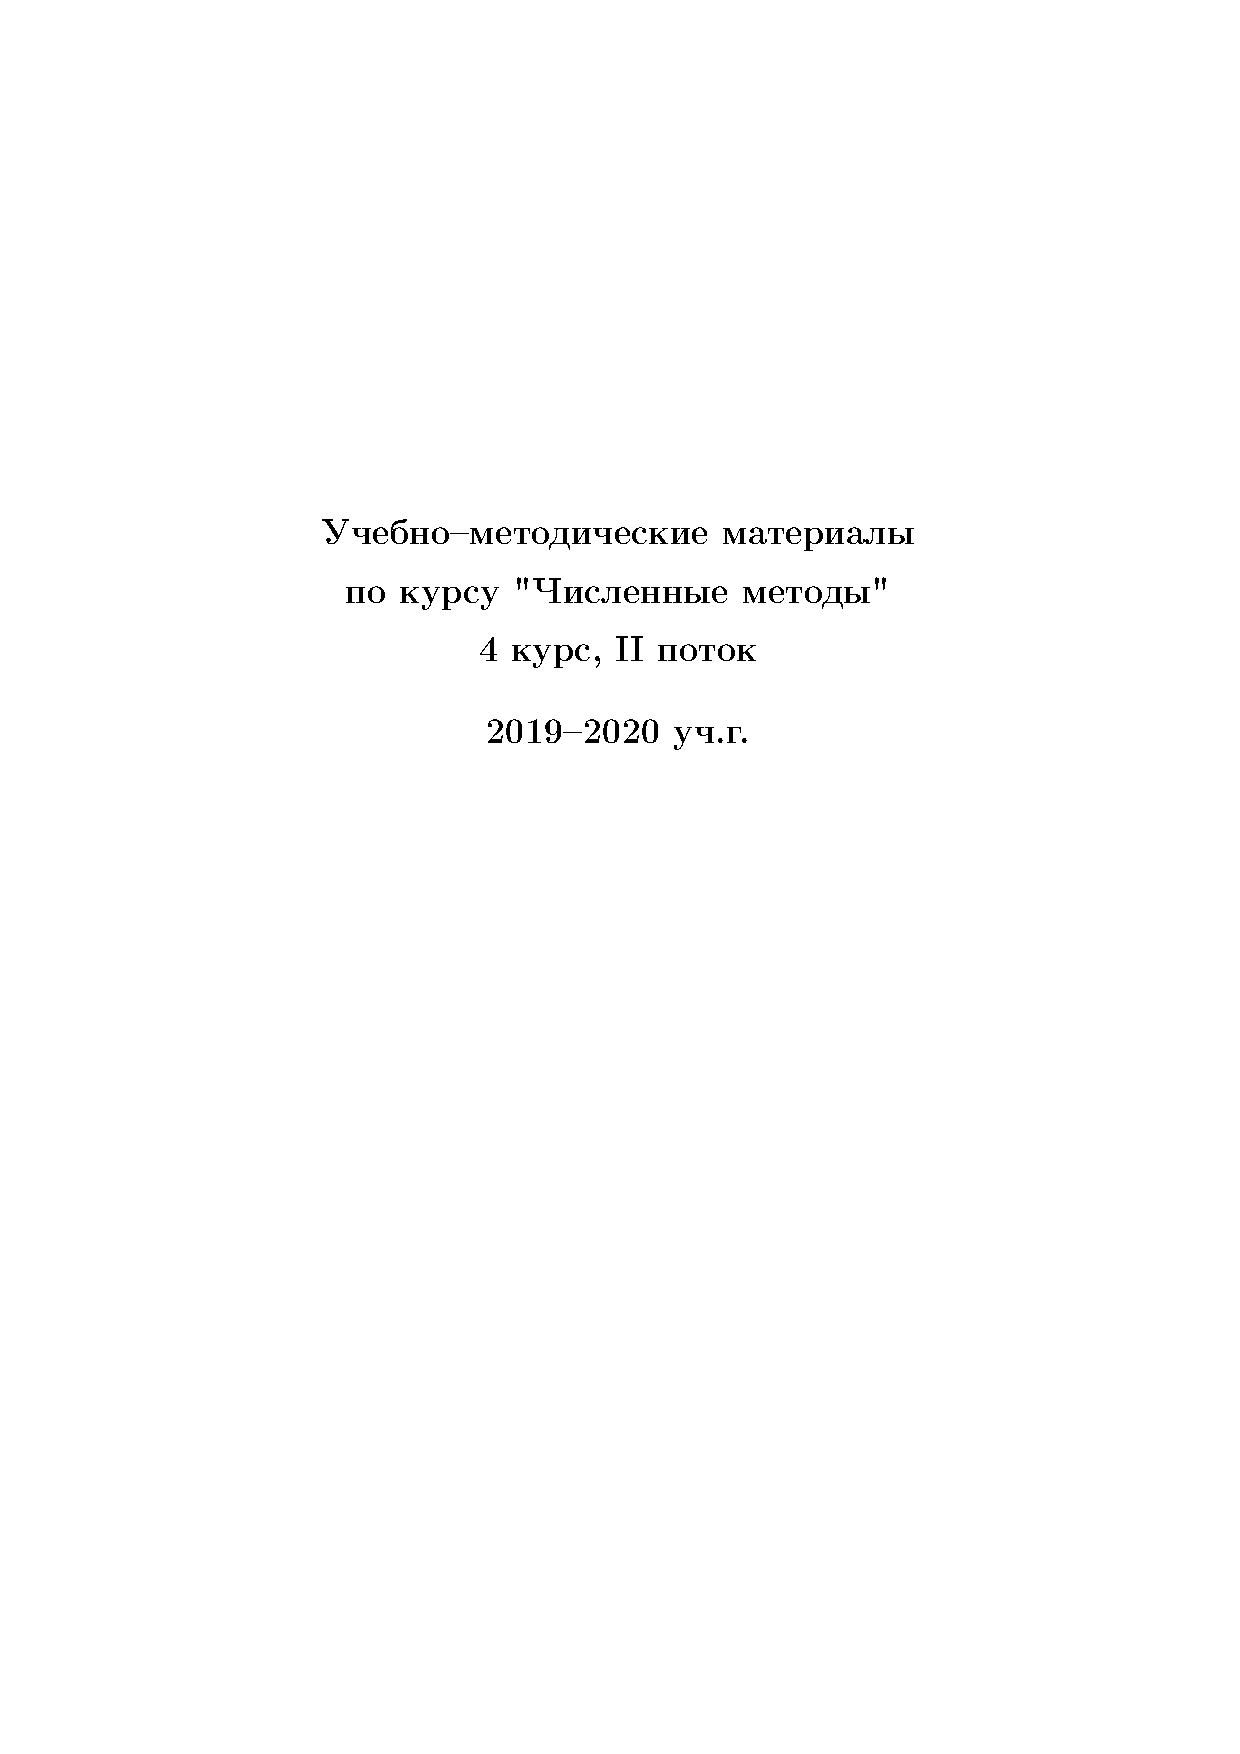
\includepdf[pages=-, link, linkname = lects]{ch-m_II-20.pdf}

\end{document}
